\documentclass[../the.tex]{subfiles}

\begin{document}

\section{Mạng tích chập đầy đủ (Fully Convolutional Network):}
\label{sec:fcn}

{\fontsize{13}{12} \selectfont
Ứng dụng phân vùng ngữ nghĩa được xây dựng thao tác trực tiếp với ảnh và mạng nơ-ron tích chập nguyên thủy \gls{cnn} (Convolutional Neural Network) là giải pháp rất thành công ở thời điểm hiện tại khi thao tác với các loại ảnh. Chính vì vậy, \gls{cnn} thường được sử dụng làm điểm tựa để nghiên cứu về vấn đề trên.}

{\fontsize{13}{12} \selectfont
Theo lý thuyết, mạng nơ-ron tích chập nguyên thủy \cite{NIPS2012_4824} là sự tổ hợp hợp lý các lớp tích chập (Convolution layer), lớp phi tuyến (Nonlinear layer) và lớp thăm dò (Pooling layer) với mỗi lớp sẽ đảm nhiệm những vai trò tính toán chuyên biệt nhằm rút lấy đặc trưng (Feature Learning), sau đó sẽ đưa qua bộ phân lớp (Classification) để xuất ra một véc-tơ chứa xác suất hay khả năng đối tượng đầu vào thuộc từng lớp đó. }

\bigskip

{\fontsize{13}{12} \selectfont
\begin{figure}[H]
\centering
	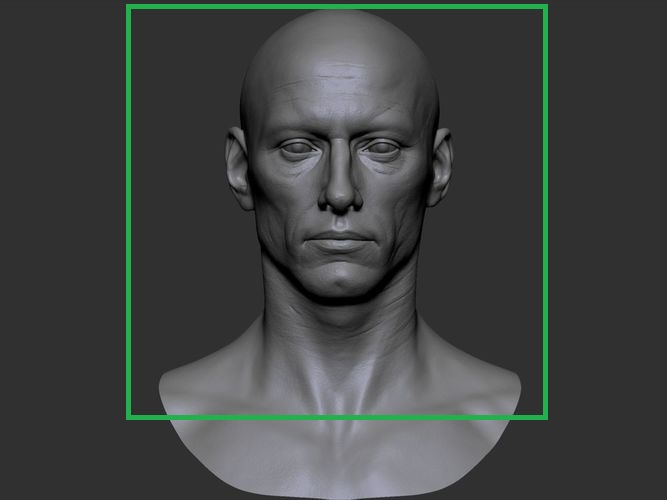
\includegraphics[scale=0.3]{cnn.jpeg}
	\caption{Mạng nơ-ron tích chập truyền thống [Nguồn: towardsdatascience.com)]}
	\label{fig:cnn_traditional}
\end{figure}}
\bigskip
\bigskip


\subsection{Bộ giảm mẫu - mã hóa (Downsampling - Encoder):}
\label{sec:encoder}


\end{document}